\documentclass[10pt]{article}
\usepackage[english]{babel}
\usepackage{../../../meta-inf/lib/naproche}
\usepackage{amssymb}
\usepackage{mathtools} % for \coloneq

\usepackage{stex-highlighting}
\providebool{emph} % "\newbool{emph}" does not work...
\setbool{emph}{false}
\colorlet{emphcolor}{violet}
\let\oldemph\emph
\renewcommand\emph[1]{\setbool{emph}{true}\ifbool{forthel}{\textcolor{emphcolor}{\itshape#1}}{\oldemph{#1}}\setbool{emph}{false}}
\renewcommand{\varemph}[1]{\ifbool{emph}{\textcolor{emphcolor}{#1}}{\textcolor{black}{#1}}}

\usepackage[right=6cm,left=3cm,bottom=3cm,marginparwidth=5cm]{geometry}

\usepackage{fancyhdr}
\renewcommand{\sectionmark}[1]{\markboth{#1}{}} 
\def\libarchive{}
\pagestyle{fancy}
\fancyhead[L]{\libarchive}
\fancyhead[C]{\nouppercase\leftmark}  % section title
\fancyhead[R]{\thepage}               % page number
\fancyfoot[C]{}                       % No page number in footer

\usepackage[nobottomtitles]{titlesec}
\titlespacing*{\section}{0pt}{30pt}{0pt}
\titlespacing*{\subsection}{0pt}{30pt}{0pt}
\titlespacing*{\subsubsection}{0pt}{30pt}{0pt}

\documentclass[12pt,oneside]{book}

\usepackage[foundations]{../../lib/tex/naproche}
\usepackage{../../lib/tex/libraries}
\usepackage{graphicx}
\usepackage{float}
\usepackage{caption}
\usepackage{footnote}

\makesavenoteenv{tabular} % Make footnotes work in tabular environments


\title{Foundations of Mathematics}
\author{Marcel Schütz}
\date{2022}

\begin{document}
  \maketitle

  \tableofcontents

  \begin{figure}[H]
    \centering
    \fbox{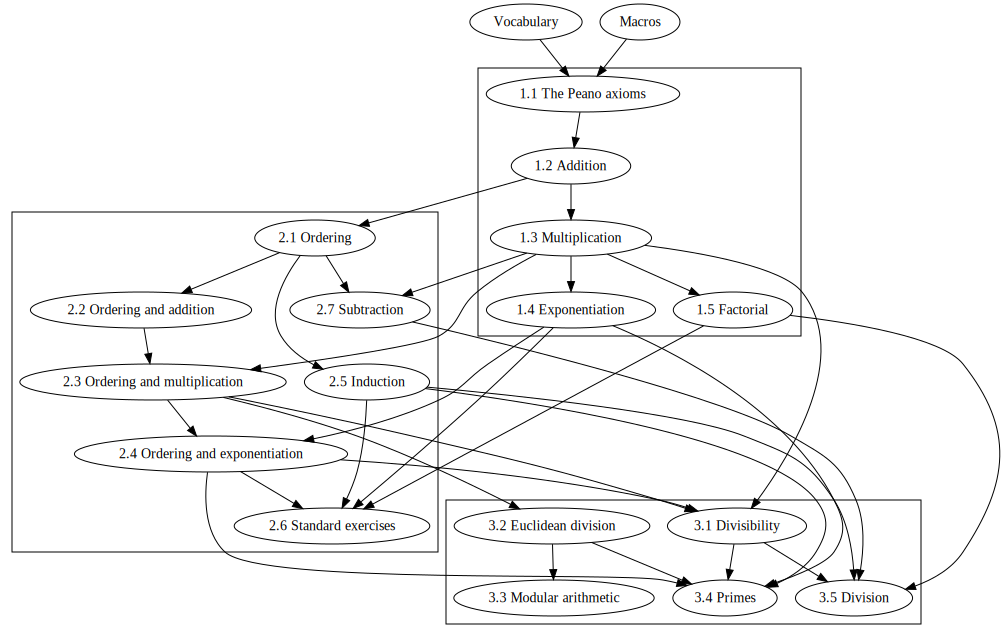
\includegraphics[width=0.9\linewidth]{./dependency-graph/graph.png}}
    \caption*{Interdependencies of the chapters}
  \end{figure}


  \section*{Introduction}

  This is a library providing a foundation of mathematics based on a
  Kelley-Morse like class theory with urelements.
  It introduces common operations on classes like unions or intersections
  (\cref{chapter:classes}) together with detailed proofs of their algebraic
  properties (\cref{chapter:computation-laws-for-classes}), the symmetric
  difference of two classes (\cref{chapter:symmetric-difference}) and the
  notions of ordered pairs and Cartesian products
  (\cref{chapter:pairs-and-products}) as well as proofs of the algebraic
  properties of the latter (\cref{chapter:computation-laws-for-products}).
  Moreover, it provides common operations on maps (\cref{chapter:maps}), various
  properties of images and preimages (\cref{chapter:image-and-preimage}) and the
  notions of injectivity, surjectivity, bijectivity
  (\cref{chapter:injections-surjections-bijections}) and invertibility of maps
  (\cref{chapter:invertible-maps}).
  The library provides an axiom system characterizing sets (\cref{chapter:sets})
  and, furthermore, it covers the notions of binary relations
  (\cref{chapter:binary-relations}), fixed-points of subset preserving maps
  (\cref{chapter:fixed-points}), including and equinumerosity
  (\cref{chapter:equinumerosity}).

  As two famous results it includes the Knaster-Tarski fixed point theorem
  (\cref{FOUNDATIONS_12_8420450166112256}) and the Cantor-Schröder-Bernstein
  theorem (\cref{FOUNDATIONS_13_1913663275401216}).

  \paragraph*{Usage.}
  At the very beginning of each chapter you can find the name of its source
  file, e.g. \path{foundations/sections/01_classes.ftl.tex} for
  \cref{chapter:classes}. This filename can be used to import the chapter via
  \Naproche's \texttt{readtex} instruction to another ForTheL text, e.g.:
  \begin{center}
    \verb`[readtex \path{foundations/sections/01_classes.ftl.tex}]`
  \end{center}

  \paragraph*{Checking times.}
  The checking times for each of the chapters may vary from computer to
  computer, but on mid-range hardware they are likely to be similar to those
  given in table below:

  \begin{center}
    \begin{tabular}{c|c|c}

      & \multicolumn{2}{c}{\textbf{Checking time}}
      \\
      \textbf{Chapter}
      & \textbf{without dependencies}     & \textbf{with dependencies}
      \\ \hline
      \ref{chapter:classes}
      & 00:04 min                         & 00:04 min
      \\
      \ref{chapter:computation-laws-for-classes}
      & 00:12 min                         & 00:16 min
      \\
      \ref{chapter:symmetric-difference}
      & 00:32 min                         & 00:48 min
      \\
      \ref{chapter:pairs-and-products}
      & 00:08 min                         & 00:12 min
      \\
      \ref{chapter:computation-laws-for-products}
      & 01:36 min                         & 01:56 min
      \\
      \ref{chapter:maps}
      & 01:13 min                         & 01:25 min
      \\
      \ref{chapter:image-and-preimage}
      & 01:28 min                         & 02:53 min
      \\
      \ref{chapter:injections-surjections-bijections}
      & 00:38 min                         & 02:03 min
      \\
      \ref{chapter:invertible-maps}
      & 02:20 min                         & 04:23 min
      \\
      \ref{chapter:sets}
      & 02:17 min                         & 06:40 min
      \\
      \ref{chapter:binary-relations}
      & 00:14 min                         & 06:54 min
      \\
      \ref{chapter:fixed-points}
      & 00:33 min                         & 07:13 min
      \\
      \ref{chapter:equinumerosity}
      & 01:48 min                         & 09:01 min
    \end{tabular}
  \end{center}


  \subfile{sections/01_classes.ftl.tex}
  \subfile{sections/02_computation-laws-for-classes.ftl.tex}
  \subfile{sections/03_symmetric-difference.ftl.tex}
  \subfile{sections/04_pairs-and-products.ftl.tex}
  \subfile{sections/05_computation-laws-for-products.ftl.tex}
  \subfile{sections/06_maps.ftl.tex}
  \subfile{sections/07_image-and-preimage.ftl.tex}
  \subfile{sections/08_injections-surjections-bijections.ftl.tex}
  \subfile{sections/09_invertible-maps.ftl.tex}
  \subfile{sections/10_sets.ftl.tex}
  \subfile{sections/11_binary-relations.ftl.tex}
  \subfile{sections/12_fixed-points.ftl.tex}
  \subfile{sections/13_equinumerosity.ftl.tex}
\end{document}

\begin{document}
  \begin{imports}
    \begin{forthel}
      %[prove off][check off]
      [read \path{libraries/source/foundations/injections-surjections-bijections.ftl.tex}]
      %[prove on][check on]
    \end{forthel}
  \end{imports}


  \section*{Invertible Maps}

  \subsection*{Definitions}

  \begin{forthel}
    \begin{definition}[id=FOUNDATIONS_09_7776974319648768,printid]
      Let $f$ be a map.
      An inverse of $f$ is a map $g$ from $\range(f)$ to $\dom(f)$ such that $f(a) = b \iff g(b) = a$ for all $a \in \dom(f)$ and all $b \in \dom(g)$.
    \end{definition}
  \end{forthel}

  \begin{forthel}
    \begin{definition}[id=FOUNDATIONS_09_3430350086733824,printid]
      Let $f$ be a map.
      $f$ is invertible iff $f$ has an inverse.
    \end{definition}
  \end{forthel}

  \begin{forthel}
    \begin{lemma}[id=FOUNDATIONS_09_5108611793551360,printid]
      Let $f$ be a map and $g, g'$ be inverses of $f$.
      Then $g = g'$.
    \end{lemma}
    \begin{proof}
      We have $\dom(g) = \range(f) = \dom(g')$.

      Let us show that $g(b) = g'(b)$ for all $b \in \range(f)$.
        Let $b \in \range(f)$.
        Take $a = g'(b)$.
        Then $g(b) = a$ iff $f(a) = b$.
        We have $f(a) = b$ iff $g'(b) = a$.
        Thus $g(b) = g'(b)$.
      End.
    \end{proof}
  \end{forthel}

  \begin{forthel}
    \begin{definition}[id=FOUNDATIONS_09_6458627204317184,printid]
      Let $f$ be an invertible map.
      $f^{-1}$ is the inverse of $f$.
    \end{definition}

    Let $f$ is involutory stand for $f$ is the inverse of $f$.
    Let $f$ is selfinverse stand for $f$ is the inverse of $f$.
  \end{forthel}


  \subsection*{Basic Properties}

  \begin{forthel}
    \begin{proposition}[id=FOUNDATIONS_09_7840743571849216,printid]
      Let $A, B$ be classes and $f : A \onto B$ and $g : B \onto A$.
      Then $g$ is the inverse of $f$ iff $g \circ f = \id_{A}$ and $f \circ g = \id_{B}$.
    \end{proposition}
    \begin{proof}
      Case $g$ is the inverse of $f$.
        We have
        $\dom(g \circ f)
          = \dom(f)
          = A
          = \dom(\id_{A})$.
        For all $a \in A$ we have
        $(g \circ f)(a)
          = g(f(a))
          = a$.
        Hence $g \circ f = \id_{A}$.

        We have
        $\dom(f \circ g)
          = \dom(g)
          = B
          = \dom(\id_{B})$.
        For all $b \in B$ we have
        $(f \circ g)(b)
          = f(g(b))
          = b$.
        Hence $f \circ g = \id_{B}$.
      End.

      Case $g \circ f = \id_{A}$ and $f \circ g = \id_{B}$.
        Then $\dom(g)
          = B
          = \range(f)$
        and $\range(g)
          = A
          = \dom(f)$.
        Let $a \in \dom(f)$ and $b \in \dom(g)$.
        If $f(a) = b$ then
        $g(b)
          = g(f(a))
          = (g \circ f)(a)
          = \id_{A}(a)
          = a$.
        If $g(b) = a$ then
        $f(a)
          = f(g(b))
          = (f \circ g)(b)
          = \id_{B}(b)
          = b$.
        Hence $f(a) = b$ iff $g(b) = a$.
      End.
    \end{proof}
  \end{forthel}

  \begin{forthel}
    \begin{proposition}[id=FOUNDATIONS_09_8414736098000896,printid]
      Let $A, B$ be classes and $f : A \onto B$.
      Assume that $f$ is invertible.
      Then $f^{-1}$ is an invertible surjective map from $B$ onto $A$ such that $(f^{-1})^{-1} = f$.
    \end{proposition}
    \begin{proof}
      $f^{-1}$ is a map from $B$ to $A$.
      Indeed $\range(f) = B$ and $\dom(f) = A$.
      $f^{-1}$ is surjective onto $A$.
      Indeed for any $a \in A$ we have $f^{-1}(f(a)) = a$.
      $f^{-1}$ is the inverse of $f$.
      Thus $f \circ f^{-1} = \id_{B}$ and $f^{-1} \circ f = \id_{A}$.
      Therefore $f$ is the inverse of $f^{-1}$.
    \end{proof}
  \end{forthel}

  \begin{forthel}
    \begin{proposition}[id=FOUNDATIONS_09_4577560740495360,printid]
      Let $A, B$ be classes and $f : A \onto B$.
      Assume that $f$ is invertible.
      Then $f \circ f^{-1} = \id_{B}$ and $f^{-1} \circ f = \id_{A}$.
    \end{proposition}
    \begin{proof}
      $f^{-1}$ is a surjective map from $B$ onto $A$ .
      $f^{-1}$ is the inverse of $f$.
    \end{proof}
  \end{forthel}

  \begin{forthel}
    \begin{proposition}[id=FOUNDATIONS_09_4606651604664320,printid]
      Let $A, B$ be classes and $f : A \onto B$ and $a \in A$.
      Assume that $f$ is invertible.
      Then $f^{-1}(f(a)) = a$.
    \end{proposition}
    \begin{proof}
      We have $f^{-1}(f(a)) = (f^{-1} \circ f)(a) = \id_{A}(a) = a$.
    \end{proof}

    \begin{proposition}
      Let $A, B$ be classes and $f : A \onto B$ and $b \in B$.
      Assume that $f$ is invertible.
      Then $f(f^{-1}(b)) = b$.
    \end{proposition}
    \begin{proof}
      We have
      $f(f^{-1}(b))
        = (f \circ f^{-1})(b)
        = \id_{B}(b)
        = b$.
    \end{proof}
  \end{forthel}

  \begin{forthel}
    \begin{proposition}[id=FOUNDATIONS_09_7619151963095040,printid]
      Let $A, B, C$ be classes and $f : A \onto B$ and $g : B \onto C$.
      Assume that $f$ and $g$ are invertible.
      Then $g \circ f$ is invertible and $(g \circ f)^{-1} = f^{-1} \circ g^{-1}$.
    \end{proposition}
    \begin{proof}
      $f^{-1}$ is a surjective map from $B$ onto $A$.
      $g^{-1}$ is a surjective map from $C$ onto $B$.
      Take $h = f^{-1} \circ g^{-1}$.
      Then $h$ is a surjective map from $C$ onto $A$ (by \printref{FOUNDATIONS_08_8542698338254848}).
      $g \circ f$ is a map from $A$ to $C$.

      Let us show that $((g \circ f) \circ h) = \id_{C}$.
        We have $f \circ (f^{-1} \circ g^{-1}) = (f \circ f^{-1}) \circ g^{-1}$.
        Indeed $f \circ (f^{-1} \circ g^{-1})$ and $(f \circ f^{-1}) \circ g^{-1}$ are maps of $C$.
        $f \circ h$ is a map from $C$ to $B$.
        Hence
        \[  (g \circ f) \circ h                           \]
        \[    = g \circ (f \circ h)                       \]
        \[    = g \circ (f \circ (f^{-1} \circ g^{-1}))   \]
        \[    = g \circ ((f \circ f^{-1}) \circ g^{-1})   \]
        \[    = g \circ (\id_{B} \circ g^{-1})            \]
        \[    = g \circ g^{-1}                            \]
        \[    = \id_{C}.                                  \]
      End.

      Let us show that $h \circ (g \circ f) = \id_{A}$.
        We have $(f^{-1} \circ g^{-1}) \circ g = f^{-1} \circ (g^{-1} \circ g)$.
        $g \circ f$ is a map from $A$ to $C$.
        Hence
        \[  h \circ (g \circ f)                           \]
        \[    = (h \circ g) \circ f                       \]
        \[    = ((f^{-1} \circ g^{-1}) \circ g) \circ f   \]
        \[    = (f^{-1} \circ (g^{-1} \circ g)) \circ f   \]
        \[    = (f^{-1} \circ \id_{B}) \circ f            \]
        \[    = f^{-1} \circ f                            \]
        \[    = \id_{A}.                                  \]
      End.

      Thus $h$ is the inverse of $g \circ f$.
      Indeed $g \circ f$ is a surjective map from $A$ onto $C$ and $h$ is a surjective map from $C$ onto $A$.
    \end{proof}
  \end{forthel}

  \begin{forthel}
    \begin{proposition}[id=FOUNDATIONS_09_6374884963778560,printid]
      Let $A, B$ be classes and $f : A \onto B$ and $X \subseteq A$.
      Assume that $f$ is invertible.
      Then $f \restriction X$ is invertible and $(f\restriction X)^{-1} = f^{-1} \restriction (f_{*}(X))$.
    \end{proposition}
    \begin{proof}
      $f \restriction X$ is a surjective map from $X$ onto $f_{*}(X)$.
      Take $g = f^{-1} \restriction (f_{*}(X))$.
      Then $g$ is a map of $f_{*}(X)$.

      Let us show that $X \subseteq \range(g)$.
        Let $a \in X$.
        Then $f(a) \in f_{*}(X)$.
        Hence $g(f(a)) = f^{-1}(f(a)) = a$.
        Thus $a$ is a value of $g$.
      End.

      Let us show that $\range(g) \subseteq X$.
        Let $a \in \range(g)$.
        Take $b \in f_{*}(X)$ such that $a = g(b)$.
        Take $c \in X$ such that $b = f(c)$.
        Then $a
          = (f^{-1} \restriction (f_{*}(X)))(b)
          = f^{-1}(b)
          = f^{-1}(f(c))
          = c$.
        Hence $a \in X$.
      End.

      Hence $\range(g) = X$.
      Thus $g$ is a surjective map onto $X$.

      Let us show that $g((f \restriction X)(a)) = a$ for all $a \in X$.
        Let $a \in X$.
        Then $g((f \restriction X)(a))
          = g(f(a))
          = (f^{-1} \restriction (f_{*}(X)))(f(a))
          = f^{-1}(f(a))
          = a$.
      End.

      Let us show that $((f \restriction X)(g(b))) = b$ for all $b \in f_{*}(X)$.
        Let $b \in f_{*}(X)$.
        Take $a \in X$ such that $b = f(a)$.
        We have $g(b)
          = g(f(a))
          = (f^{-1} \restriction (f_{*}(X)))(f(a))
          = f^{-1}(f(a))
          = a$.
        Hence $(f \restriction X)(g(b))
          = (f \restriction X)(a)
          = f(a)
          = b$.
      End.

      Thus $g \circ (f \restriction X) = \id_{X}$ and $(f \restriction X) \circ g = \id_{f_{*}(X)}$.
      Therefore $g$ is the inverse of $f \restriction X$.
    \end{proof}
  \end{forthel}

  \begin{forthel}
    \begin{proposition}[id=FOUNDATIONS_09_7726021377785856,printid]
      Let $A, B$ be classes and $f : A \onto B$ and $Y \subseteq B$.
      Assume that $f$ is invertible.
      Then \[ f^{*}(Y) = (f^{-1})_{*}(Y). \]
    \end{proposition}
    \begin{proof}
      We have $(f^{-1})_{*}(Y) = \{ f^{-1}(b) \mid b \in Y \}$ and $f^{*}(Y) = \{ a \in A \mid f(a) \in Y \}$.

      Let us show that $f^{*}(Y) \subseteq (f^{-1})_{*}(Y)$.
        Let $a \in f^{*}(Y)$.
        Take $b \in Y$ such that $b = f(a)$.
        Then $f^{-1}(b) = f^{-1}(f(a)) = a$.
        Hence $a \in (f^{-1})_{*}(Y)$.
      End.

      Let us show that $f^{-1}_{*}(Y) \subseteq f^{*}(Y)$.
        Let $a \in f^{-1}_{*}(Y)$.
        Take $b \in Y$ such that $a = f^{-1}(b)$.
        Then $f(a) = f(f^{-1}(b)) = b$.
        Hence $a \in f^{*}(Y)$.
      End.
    \end{proof}
  \end{forthel}

  \begin{forthel}
    \begin{corollary}[id=FOUNDATIONS_09_8607784268464128,printid]
      Let $A, B$ be classes and $f : A \onto B$ and $b \in B$.
      Assume that $f$ is invertible.
      Then \[ f^{*}(\set{b}) = \set{f^{-1}(b)}. \]
    \end{corollary}
    \begin{proof}
      $f^{*}(\set{b}) = f^{-1}_{*}(\set{b})$.
      We have $f^{-1}_{*}(\set{b}) = \{ f^{-1}(c) \mid c \in \set{b} \}$.
      Hence $f^{-1}_{*}(\set{b}) = \set{f^{-1}(b)}$.
    \end{proof}
  \end{forthel}

  \begin{forthel}
    \begin{proposition}[id=FOUNDATIONS_09_6777575974109184,printid]
      Let $A, B$ be classes and $f : A \onto B$.
      Then $f$ is invertible iff $f$ is injective.
    \end{proposition}
    \begin{proof}
      Case $f$ is invertible.
        Let $a, b \in A$.
        Assume $f(a) = f(b)$.
        Then $a = f^{-1}(f(a)) = f^{-1}(f(b)) = b$.
      End.

      Case $f$ is injective.
        Define $g(b) =$ ``choose $a \in A$ such that $f(a) = b$ in $a$'' for
        $b \in B$.
        Then $g$ is a map from $B$ to $A$.
        For all $a \in A$ we have $a = g(f(a))$.
        Hence $g$ is a surjective map from $B$ onto $A$.
        For all $a \in A$ we have $g(f(a)) = a$.
        For all $b \in B$ we have $f(g(b)) = b$.
        Hence $g$ is the inverse of $f$.
      End.
    \end{proof}
  \end{forthel}

  \begin{forthel}
    \begin{corollary}[id=FOUNDATIONS_09_5708971514003456,printid]
      Let $A, B$ be classes and $f : A \onto B$.
      Assume that $f$ is invertible.
      Then $f^{-1}$ is a bijection between $B$ and $A$.
    \end{corollary}
    \begin{proof}
      $f^{-1}$ is a surjective map from $B$ onto $A$.
      $f^{-1}$ is invertible.
      Hence $f^{-1}$ is injective.
      Therefore $f^{-1}$ is a bijection between $B$ and $A$.
    \end{proof}
  \end{forthel}


  \subsection*{Involutions}

  \begin{forthel}
    \begin{definition}[id=FOUNDATIONS_09_7282039688527872,printid]
      Let $A$ be a class.
      An involution on $A$ is a selfinverse map $f$ on $A$.
    \end{definition}
  \end{forthel}

  \begin{forthel}
    \begin{proposition}[id=FOUNDATIONS_09_7944474185433088,printid]
      Let $A$ be a class.
      $\id_{A}$ is an involution on $A$.
    \end{proposition}
    \begin{proof}
      We have $\id_{A} \circ \id_{A} = \id_{A}$.
      Hence $\id_{A}$ is selfinverse.
    \end{proof}
  \end{forthel}

  \begin{forthel}
    \begin{proposition}[id=FOUNDATIONS_09_6897019612299264,printid]
      Let $A$ be a class and $f, g$ be involutions on $A$.
      Then $g \circ f$ is an involution on $A$ iff $g \circ f = f \circ g$.
    \end{proposition}
    \begin{proof}
      Case $g \circ f$ is an involution on $A$.
        Then $(g \circ f)^{-1}
          = f^{-1} \circ g^{-1}
          = f \circ g$
        (by \printref{FOUNDATIONS_09_7619151963095040}).
        Indeed $f$ and $g$ are invertible and surjective onto $A$.
      End.

      Case $g \circ f = f \circ g$.
        $f \circ f$, $f \circ g$ and $f \circ g$ are maps on $A$.
        Hence
        \[  (g \circ f) \circ (g \circ f)       \]
        \[    = (g \circ f) \circ (f \circ g)   \]
        \[    = ((g \circ f) \circ f) \circ g   \]
        \[    = (g \circ (f \circ f)) \circ g   \]
        \[    = (g \circ \id_{A}) \circ g       \]
        \[    = g \circ g                       \]
        \[    = \id_{A}.                        \]
        Thus $g \circ f$ is selfinverse.
      End.
    \end{proof}
  \end{forthel}

  \begin{forthel}
    \begin{corollary}[id=FOUNDATIONS_09_5958206868160512,printid]
      Let $A$ be a class and $f$ be an involutions on $A$.
      Then $f \circ f$ is an involution on $A$.
    \end{corollary}
  \end{forthel}

  \begin{forthel}
    \begin{proposition}[id=FOUNDATIONS_09_2314262743613440,printid]
      Let $A$ be a class and $f$ be an involution on $A$.
      Then $f$ is a permutation of $A$.
    \end{proposition}
    \begin{proof}
      $f$ is an invertible map of $A$ that surjects onto $A$.
      Hence $f$ is a bijection between $A$ and $A$.
      Thus $f$ is a permutation of $A$.
    \end{proof}
  \end{forthel}
\end{document}
